\acresetall
%%=========================================
\chapter{Background}\label{ch:background}
To better comprehend the models that are presented in this thesis, an understanding of some central theories within the field of language evolution is necessary. This chapter will present language evolution, language games, Schwartz' theory of basic human values, graph theory, social network theory and \acp{ga}.
%This chapter will present theories within the field of language evolution, graph theory, social network theory, Schwartz' theory of basic human values, and \acp{ga}.\todo{skriv hvorfor disse tingene tas opp i teorien også.}todo{Legg in Schwartz i teori kapittelet}.

\section{Language Evolution}
Biolinguists, evolutionary linguists, and sociolinguists all have different theories on how the human language evolved. The biolinguists think that the evolution of human language can be explained through biological evolution, and they argue that the composition of a language, e.g. the sentence structure subject-verb-object in English, can be explained through a language acquisition device which can understand a universal grammar \citep{chomsky1965some}.

The evolutionary linguists believe that language evolved through natural selection in a Darwinian manner. \citet{pinker1994regular} proposed an explanation for the evolution of human language by looking at the evolution of non-human animals' abilities. They suggested that, just like bats evolved the ability to perceive their environment through echolocation, humans evolved the ability to understand and learn cognitive-functional linguistics.

In recent years, there has been a discussion concerning the importance of individual learning and how big of an impact culture and society has on individual learning. Sociolinguists believe that language evolution is affected by society and culture \citep{tomasello2003makes}. Their theory has been strengthened by the use of computational models of simplified social networks. These models show that social networks affect language evolution.

\label{EvoltionaryForces}
There are three forces that are believed to affect language evolution: biological evolution, cultural evolution, and social evolution, see Figure~\ref{fig:LanguageForces}. To fully understand the theories on language evolution, the theories have to be viewed in the light of these three forces.

Biological evolution is the slowest force, working on a \textit{phylogenetic} time scale. It involves how an individual improves its abilities to learn and process language in order to survive and reproduce.
Cultural evolution works on a historical time scale, called the \textit{glossogenetic} time scale. In cultural evolution, the change is viewed upon unique languages that exist within a society. It concerns how the features of the language get culturally transferred from one person to another, and from one generation to another.
Social evolution is looked at during one person's lifetime, and the evolution is said to work on an \textit{ontogenetic} time scale. It concerns how an individual learns a language. A person's ability to learn the language is an important factor as to how a language is built up. Newborns' ability to quickly go from having no language at all to being able to speak several languages indicates that humans and language have co-evolved so that human language will be easy to learn during infancy \citep{tomasello2003makes}.

\begin{figure}[ht]
    \centering
    \includegraphics[scale=0.7]{LanguageForces}
    \caption[Illustration of the three forces of language evolution.]{Illustration of the three forces of language evolution that are believed to affect language evolution: biological evolution, cultural evolution, and social evolution.}
    \label{fig:LanguageForces}
\end{figure}

\subsection{Origin of Language}
No one knows exactly how or when humans began communicating. In order for language to have emerged, there had to be a need for communication. For example, if one person saw a deer approaching, that person would want to communicate that to the others so that they could go and hunt together. Situations like this, where communication was beneficial, is likely to have arisen often. Most linguists agree upon the theory that the first human form of communication was holistic, i.e. simple utterances and physical gestures, and was used to express a reaction to concepts such as hunt or run \citep{christiansen2003language}. How a holistic language evolved into the syntactical language used today is not known \citep{bickerton2007language}.

\subsection{Baldwin Effect}
The Baldwin effect is based on the idea that the traits an individual learns during its lifetime can guide evolution \citep{baldwin1896new}. Learning a skill comes with a cost, so if that skill is very important, the individuals with an innate ability to learn this skill have an advantage over the others. If the cost of acquiring the skill stays high and the skill remains important over time, individuals that easily master the skill will be favoured in natural selection. For example, the skill of making a fire, if this skill were to become instinctive, the population as a whole would save a lot of time not having to teach everyone how to make fire. The individuals that learn the skill easily have an advantage because they can use the spare time doing other essential tasks, like hunting for food. If the selection pressure is high enough and the cost of learning the art of making a fire is high during several generations, the Baldwin effect states that the population will eventually consist of individuals that easily learn how to make a fire.

Many researchers have experimented with the Baldwin effect during recent years. \citet{lipowska2011naming} argues that the results from her model show that the learned traits during an individual's lifetime have an effect on language evolution, meaning that the Baldwin effect has an effect on language evolution. \citet{zollman2010plasticity} also conclude that their model indicates that the Baldwin effect is influencing the evolution of language. \citet{chater2010language} argue that, based on their results, the Baldwin effect may have an influence on parts of language evolution. However, the parts of the language that change consistently, such as word order and morphology, i.e. the structure of words, would have a too low selection pressure for the Baldwin effect to have an impact on them.

%%%%%%%%%%%%%%%%%%%%%%%%%%%%%%%%%%%%%%%%%%%%%%%%%%%%%%%%%%%%%%%%%%%%%%%%%%%%%%%%%%%%%%%%%%%%%%%%%%%%%%%%%%%%%%%%%%%%%%%%%%%%%%%%%%%%%%%%%%%

\section{Language Games}
Language games are games where artificial agents interact with each other and try to understand each other. For the agents to understand each other, they need to reach a state where their individual languages are similar. This similarity is reached by the agents conversing and changing their respective vocabularies based on what the other agent utters.

Two agents are picked out, traditionally at random, and one of the agents gets the role of \textit{hearer} and the other agent is the \textit{speaker}. The speaker then utters something about a concept. If the hearer understands the utterance, the conversation is labelled as a success, and if the hearer did not understand, the conversation is labelled as a failure. If the speaking agent does not have any way of describing the concept perceived, it has the ability to make up new words in order to describe the concept. 

Language games have become a standard method of simulating language within the field of computer simulations of language evolution. Many variations of language games have been designed: naming games, spatial naming games, and signalling games will be presented in the following subsections.

\subsection{Naming Games}
Simple naming games typically have a language without grammar, and all conversations occur without an environment. All agents have a vocabulary containing words they have heard or invented during conversations with other agents. Conversations occur between two agents, they attempt to agree upon an utterance for an object they both have perceived. If both agents can agree upon an utterance, the conversation is redeemed as a success, and that utterance becomes more likely to be used again for both agents. If they cannot agree, the hearing agent adds the new word to its vocabulary and the speaking agent decreases the probability of that word being used again. Words that have not been used successfully in a long time are eventually removed from the agent's vocabulary.

During the first generations there will be many unsuccessful conversations, leading to words being spread around in the population giving all agents a large vocabulary. When the agents have added enough words to their vocabularies, some conversations will be successful. This will lead to agents removing their least successful words. If the simulation is given enough time, the agents may reach a consensus on almost all words. However, reaching a consensus on the last words seems to require some element of chance \citep{steels1997synthetic}.

Naming games are often used to analyse cultural transmission between agents of the same generation. \citeauthor{lipowska2011naming} made a computational simulation using naming games which analysed the cultural transmission over several generations. This model will be reviewed in section \ref{sec:Lipowska}.

\subsection{Spatial Naming Games}\label{SpatNamingGame}
Spatial naming games are a form of naming games where all conversations are set in the same environment. The speaking agent describes its understanding of the environment to the listener. If the listener agrees with the description of the environment, the conversation is viewed upon as a success. If the agents do not agree, the conversation is deemed as a failure. As with normal simple games, the goal is that all agents reach a consensus. \citeauthor{gong2011simulating} simulated agents that tried to reach a consensus by building up a compositional language. His work will be examined further in section \ref{sec:Gong}.

\subsection{Signalling Games}
Signalling games simulate a compositional language using an \ac{ann}. The signal uttered is the output of an agent's \ac{ann}. The output will normally be a sequence of numerical values where the order of the numbers represents a sentence in natural language. This abstraction makes it easier to study compositional languages \citep{munroe2002learning, suzuki2008learning}. \citeauthor{munroe2002learning} made a signalling game where the language was evolved by agents walking around in a world of mushrooms. The agents' task was to reach a consensus concerning which mushrooms were edible and which were not. This was done by evolving a language from \acp{ann}. The computational model using signalling games made by \citeauthor{munroe2002learning} will be examined further in section \ref{sec:Munroe}.

%%%%%%%%%%%%%%%%%%%%%%%%%%%%%%%%%%%%%%%%%%%%%%%%%%%%%%%%%%%%%%%%%%%%%%%%%%%%%%%%%%%%%%%%%%%%%%%%%%%%%%%%%%%%%%%%%%%%%%%%%%%%%%%%%%%%%%%%%%%%%%%%

\section{Schwartz's Theory of Basic Values}\label{SchwartzBasicValues}
There is no doubt that personality affects a person's social network. Personality is so complex that even making a simplistic model of it might seem impossible. \citet{schwartz1992unniversals} presents a theory which models personalities by figuring out which of the types of values are most important to a person.

\subsection{Model}
\textit{The theory of Basic Values} presents ten values that all are based on one or more of the three ''universal requirements of human existence'' \citep{schwartz2012overview}. These requirements are:

\begin{enumerate}
    \item Needs of individuals as biological organisms.
    \item Necessity of coordinated social interaction.
    \item Survival and welfare needs of groups.
\end{enumerate}

Humans need to express fitting goals to other humans in order to cooperate with others and survive. Values represent these goals and language is how these values are communicated to others. The ten values in Schwartz’s theory are:

\begin{enumerate}
    \item \textbf{Self-direction}: A person that values self-direction highly has independent thought and exploring as goals. Self-direction comes from the need for control and independence.
    
    \item \textbf{Stimulation}: Goals that are induced from the stimulation value are challenge in life and excitement. Stimulation stems from the need for variation in order to keep a positive activation level.
    
    \item \textbf{Hedonism}: Pleasure and appreciation of life are goals people with a priority on Hedonism has. Hedonism comes from the enjoyment that stems from fulfilling needs. 
    
    \item \textbf{Achievement}: A person that values achievement highly has personal success by displaying competence to others as goal. The achievement values come from the fact that proficient actions are needed in order to survive and for social groups to reach their goals.
    
    \item \textbf{Power}: The goals of someone that values power are social status and control. Social settings seem to require people to have different statuses.
     
    \item \textbf{Security}: Safety and stability are the goals of someone that believes security is an important value. Security values work on both a personal level and a social level, e.g. family, nationality.
    
    \item \textbf{Conformity}: Goals that are induced from the conformity value are restraint of actions and self-discipline. Conformity stems from that individuals could have inclinations to perform actions that work against the better of the group. A person which highly values conformity does not want to perform actions that work against the better of the group.
    
    \item \textbf{Tradition}: The goals of someone with the tradition value are respect and commitment. Groups tend to develop common practises and beliefs that bind them together. These practises become traditions and symbolise that the people in the group are connected and working for the group's survival. 
    
    \item \textbf{Benevolence}: The goal of someone that values benevolence is caring about the welfare of others. Benevolence comes from requirements of how groups work. In order for a group to function, the people in it need to care about each other. This value creates feelings towards others such as friendship and love.
    
    \item \textbf{Universalism}: Understanding and protection for all people and for nature are the goals of someone that believes universalism is an important value. Universalism stands in contrast to benevolence, which focuses on the welfare of the group exclusively. These values activate when people become aware of other groups and how fragile nature is. 
\end{enumerate}

According to Schwartz, values have six features that make it possible to figure out which goals a person has based on how a person prioritises the ten values. By figuring out a person's goals and assuming that a rational person is trying to fulfil those goals, it is possible to anticipate the actions a person decides to perform. When one knows a person's goals and can anticipate someone's actions, it is fair to claim that one knows the person's personality. The six features are:
\begin{enumerate}
    \item When a value is activated, a feeling associated with the value and situation emerges.
    \item A person’s values indicate which goals the person has. 
    \item Values is a general guideline that indicates how a person will act in many different situations.
    \item Values are used to evaluate possible actions. Which actions are good or bad is decided through someone's values. These evaluations are usually performed subconsciously.
    \item A person’s values are ordered after importance.
    \item The importance of the values guides a person’s actions. Almost all situations trigger several values, so the importance of the values compared to each other affects which action is chosen.
\end{enumerate}
All values have these features. What separates the values are the goals they are connected to. 

To display the relations between the values, Schwartz made a circular model of them, see Figure~\ref{fig:TenValuesSchwartz}. The figure is divided into four categories that display the values that work towards similar goals. The categories are openness to change, self-enhancement, self-transcendence, and conservation. The values of the openness to change category contradict the values of the conservation category, while the self-enhancement category contradicts the self-transcendence category. Hedonism is split between openness to change and self-enhancement because it relates to both. The farther the values are apart from each other, the more contradictory they are. Values that are opposite to each other are therefore completely contradictory values. E.g. Conformity and tradition both completely contradict stimulation and hence both are placed opposite to stimulation. Schwartz thought that conformity is slightly more contradictory to stimulation than tradition is, so conformity was placed innermost of the two.

\begin{figure}
    \centering
    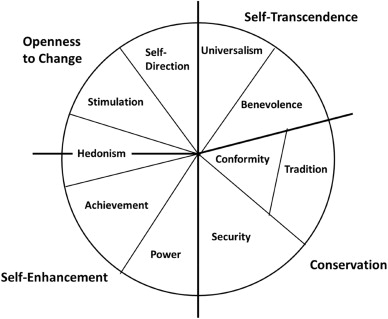
\includegraphics{TenValues}   
    \caption[The ten values from \textit{the Schwartz Theory of Basic Values}.]{The ten values from \textit{the Schwartz Theory of Basic Values}: self-direction, stimulation, hedonism, achievement, power, security, conformity, tradition, benevolence, and universalism. The circle is divided into four categories: openness to change and conservation, which represent the contradictories independence and obedience respectively, and self-transcendence and self-enhancement, which represent the contradictories interest in welfare of others and interest in welfare of oneself respectively. Values that work towards similar goals are placed in the same category \citep{schwartz2012overview}.}
    \label{fig:TenValuesSchwartz}
\end{figure}

\subsection{The Schwartz Value Survey}
In order to figure out how people prioritised their values, a survey was made by \citet{schwartz2012overview}. The survey made personality related statements and the participants answered how well the statement fitted their personality. Based on the results each of the ten values are assigned with a numerical value indicating how important that value is to the participant. The exact numerical value of the values is not what is important, it is their importance in relation to one another that matters. Normalisation is used on the ten values to scale them. 

The survey was answered by people from all over the world with many different backgrounds. A pattern in the prioritising of the values was found. It was found that benevolence, universalism, and self-direction were the most important values, while power, stimulation, and tradition were the least important ones. Almost all nations in which the study was conducted had these results. According to Schwartz, this indicates that the way people work and the way people are affected by society is quite similar in many different cultures.

%%%%%%%%%%%%%%%%%%%%%%%%%%%%%%%%%%%%%%%%%%%%%%%%%%%%%%%%%%%%%%%%%%%%%%%%%%%%%%%%%%%%%%%%%%%%%%%%%%%%%%%%%%%%%%%%%%%%%%%%%%%%%%%%%%%%%%%%%%%%%%%%%%%%%%%%%%%%%%%%%%%%%%%%%%%%%%%%%%%%%%%%%%%

\section{Graph Theory}
In recent years, a few papers have presented language game models with structured networks. \citet{lipowska2011naming} used a lattice to simulate a social graph, while others have incorporated social structures into their models \citep{lekvam2014co, gong2004computational}. This section will present discrete graphs, some of their features and how they are used in social networks.

A discrete graph is a discontinuous graph where the $x$-values of its function is limited to specific intervals, for example integers. This makes the graph consist of points, and not a line like a continuous graph. These points are usually referred to as vertices. The vertices in a discrete graph are connected with edges. These edges can be associated with a weight representing the cost between two vertices or not weighted, which essentially is the same as weighting all edges with the same value. In a discrete graph cities may be represented as vertices, and the roads between them as edges. The weight of the edges between cities could represent travel time or distance between the cities. If it is possible to travel both ways along an edge, the edge is called an \textit{undirected edge}. Otherwise, if it is only possible to travel in one direction along the edge, like a one-way driven street, it is called a \textit{directed edge}. A directed graph can have up to two edges between a vertice pair, while an undirected graph can have up to one edge between a vertice pair. Figure~\ref{fig:graph} shows an example of a directed and a undirected graph. Unless otherwise specified, the graphs presented in this thesis will be undirected.

A neighbour of a vertice, $v$, in a graph is another vertice which is connected to $v$ by an edge. The number of neighbours a vertice has is called the degree of the vertice. The density of a graph, $\mathrm{DENSITY}(G)$, is the number of edges in the graph $G$ divided by the theoretical maximum edges of $G$, $\mathrm{MAX}_\mathrm{edges}(G)$. In an undirected graph $G_\mathrm{undirected}$, with vertices $V$, the maximum number of edges are
\begin{equation}\label{eq:maximumEdges}
\mathrm{MAX}_\mathrm{edges}(G_\mathrm{undirected}) = \frac{V  (V-1)}{2}
\end{equation}

Using the definition of the density of a graph from above together with Eq.~\eqref{eq:maximumEdges}, the graph's density becomes
\begin{equation}\label{eq:densityOfGraph}
\mathrm{DENSITY}(G_\mathrm{undirected}) = \frac{2 E}{V(V-1)},
\end{equation}
where $E$ is the number of edges. Figure~\ref{fig:undirectedGraph} shows an undirected graph with three vertices: A, B and C. Vertices A and B have a degree of 1 since they have one neighbour each, while vertice C has a degree of 2 since it has two neighbours. By using Eq.~\eqref{eq:densityOfGraph}, the density of the graph becomes $2\cdot2 / (3\cdot2) = \frac{2}{3}$.

\begin{figure}[htbp]
    \centering
    \hfill
    \subfigure[\todo{FJERNE}Directed graph.]{\includegraphics[width=0.4\linewidth]{Directed_graph}\label{fig:directedGraph}}
    \hfill
    \subfigure[\todo{FJERNE}Undirected graph.]{\includegraphics[width=0.4\linewidth]{Undirected_graph}\label{fig:undirectedGraph}}
    \hfill
    \caption[The difference between a directed and an undirected graph.]{An illustration of the difference between \todo{\subref{fig:directedGraph}} a directed and \todo{\subref{fig:undirectedGraph}} an undirected graph. The circles represent vertices and the straight lines, both with and without and arrow, represent edges.}
    \label{fig:graph}
\end{figure}

\acresetall
\section{Social Networks}
A social network is a discrete graph where each vertice is a person and the edges represent how strongly two people are connected. There are a lot of factors that affect social networks and how they evolve over time. Some of these factors are language, personalities, and the environment of the social network. Several computational models that simulate the evolution of social networks have been designed. \citet{lipowska2011naming} used a lattice where each agent was restricted to only communicating with its neighbours except its first dialogues which it had with its parents. This model obviously has many limitations, such as agents cannot gain or lose connections and the connections are not weighted. 
\citet{lekvam2014co} used a social network where the edges were weighted based on the communication between the agents. It was also possible to loose and gain connections. This social network is a better representation of the real world than Lipowska's lattice, but there are other factors than just having the same language that affect a social network, like the personalities of the people in the network.

%%%%%%%%%%%%%%%%%%%%%%%%%%%%%%%%%%%%%%%%%%%%%%%%%%%%%%%%%%%%%%%%%%%%%%%%%%%%%%%%%%%%%%%%%%%%%%%%%%%%%%%%%%%%%%%%%%%%%%%%%%%%%%%%%%%%%%%%%%%%%%%%%%%%%%%%%%%%%%%%%%%%%%%%%%%%%%%%%%%%%%%%%%%

%Et lite latex-triks: Latex kan holde styr på akronymene dine, som f.eks. GA, i fila backmatter/acronyms.tex. Her legger du inn akronymet og det fulle ordet. Når du skal bruke det i teksten skriver du bare backslash ac{GA}. Første gang det dukker opp i teksten vil det fulle ordet pluss forkortelsen i parentes dukke opp, e.g. genetic algoritm (GA), mens andre, tredje, osv. gang vil kun forkortelsen dukke opp GA. For du skal ikke definere hva forkortelsen er mer enn én gang. Og ved hjelp av dette holder latex styr på det for deg. Smart, ikke sant?

\section{Genetic Algorithms} \label{GAalgorithm}
A \ac{ga} is a search algorithm based on the Darwinian principle of biological evolution. Imagine that you got the job of optimising an exam schedule at a university so that every student could take their desired combination of courses and be pleased with the exam dates. This would be impossible for humans due to the large search space. There probably does not even exist a solution where every student is pleased. In problems without a guaranteed optimal solution and with a large search space, \acp{ga} perform well.

The general structure of \iac{ga} can be seen in Figure~\ref{fig:GA}. First, a population of solutions is made, and all solutions are tested through a fitness function, which evaluates solutions and returns a fitness value that reflects how fit the solution is. Then survival selection is performed by having the fittest individuals of the population, or the best solutions, survive while the rest of the population dies. The solution that each individual represents is defined by a set of parameters, often referred to as an individual’s \textit{genome}. The genome is often represented as a bit-string. New solutions are then created by having the surviving solutions combine their genomes into new genomes by crossover, see Figure~\ref{fig:Crossover}. When a new solution is made, it has a small chance of mutation, i.e. a small alteration of the genome of the solution. Then these solutions are tested, and once again the fittest individuals survive to the next generation and get to breed.

The flow of a general \ac{ga} looks like this \citep{michalski2013machine}:
\begin{enumerate}
    \item Initialise a population $P$ of individuals with random solutions.
    \item Evaluation: Calculate the fitness of all individuals.
    \item While the highest fitness value in the population is smaller than the desired fitness value or the maximum number of iterations has not been reached, the following steps are performed:
    \begin{enumerate}
        \item Parent selection: Select which individuals to bring into the next generation based upon their fitness.
        \item Recombination: Probabilistically select two individuals based on their fitness and combine their solutions into two new solutions by using crossover.
        \item Mutation: Randomly select a few of the new individuals and let their genome mutate.
        \item Evaluation: Calculate the fitness of the new solutions.
    \end{enumerate}
\end{enumerate}


\begin{figure}[htbp]
    \centering
    \includegraphics[scale=0.7]{GA_flow}
    \caption[Flowchart of a general \ac{ga}.]{Flowchart of a general \ac{ga}. First a population is initialised with random genomes and the fitness of all individuals is calculated. As long as the highest fitness value in the population is smaller than the desired fitness value, the \ac{ga} loop is run: 1) the parents for the next generation are selected; 2) the genomes from the parents are combined by crossover to constitute the genomes of the offspring; 3) a mutation of the genome can occur; 4) the fitness of all individuals is calculated; and 5) if the highest fitness value in the population is higher than the desired fitness value, the loop is terminated, otherwise, the loop is run again.}
    \label{fig:GA}
\end{figure}

A \textit{fitness function} is a function that returns a value which gives information about how good a solution is. The fitness function of a \ac{ga} that tries to find the fastest route from one city to another would simply be the travel time of the required solution. Many problems do not have so clear objectives, or have several objectives that need to be weighted in a more complex manner.

A common issue when searching with a \ac{ga} is that if the problem at hand contains many local maxima and few global maxima, the algorithm is likely to get stuck in a local maximum because one solution is more likely to discover a local maximum than a global maximum. This solution will then often be the fittest in the population, and spread its solution to the following generations. It is called \textit{exploitation} when a good solution is spread to many agents. Exploitation allows the algorithm to perfect one solution, but it stops exploring other possibly better solutions. \textit{Exploration} is searching for new types of solutions, which is done through mutation and probabilistically choosing parents. 

One of the most common methods used in the parent selection phase is called \textit{tournament selection}. This method combines exploration, by having some randomness, and exploitation, by prioritizing the most fit individuals. First, $k$ individuals are chosen at random from all individuals. Then the individuals are sorted by their fitness, and given a rank, $r$, accordingly, i.e. the fittest individual is given $r=1$, the second fittest $r=2$, etc. Then each individual is chosen with a probability, given by
\begin{equation}
p(1-p)^r,
\end{equation}
where $p$ is a user-given probability, $0 < p < 1$, for choosing the fittest individual in a tournament. 

When two parents have been selected to mate, crossover is performed and two new individuals are created based on the parents' genomes. The most common form of crossover is performed by randomly choosing one point on the bit-string, and splitting each parent's genomes into two parts, A and B. One child receives part A from one parent and part B from the other parent. The other child receives the opposite parts. See Figure~\ref{fig:Crossover} for a simple graphic explanation of crossover. Mutation is performed on an individual with a user-given probability. Mutation is normally performed by simply flipping one bit in the bit-string.

\begin{figure}[htbp]
    \centering
    \includegraphics[scale=0.7]{crossover2}
    \caption[How crossover is used to create two offsprings from two parents with a genome represented by a bit-string.]{How crossover is used to create two offsprings from two parents with a genome represented by a bit-string. First, the genomes of the parents are divided into two parts at the same spot. Then the first part of the genome of the first parent is combined with the second part of the genome of the other parent to form the genome of the first offspring, while the first part of the genome of the second parent is combined with the second part of the genome of the first parent to form the genome of the second offspring.}
    \label{fig:Crossover}
\end{figure}
 
%%=========================================